\documentclass{article}
\usepackage[utf8]{inputenc}
\usepackage{graphicx}

\title{Analysis of Annual Mean Temperature Trends in Florida}
\author{Your Name}
\date{\today}

\begin{document}

\maketitle

\begin{abstract}
This study investigates the correlation between consecutive years' annual mean temperatures in Florida. Utilizing a robust statistical approach, we aim to uncover patterns that could inform our understanding of regional climate trends.
\end{abstract}

\section{Introduction}
In the face of changing global climates, it is imperative to understand historical temperature trends at a regional level. This study focuses on Florida, analyzing annual mean temperatures to assess the persistence and implications of observed trends.

\section{Methodology}
\subsection{Data Description}
We analyze historical annual mean temperature data for Florida, focusing on understanding year-to-year variations.

\subsection{Data Analysis Method}
The analysis involves calculating the correlation between temperatures of consecutive years using Kendall's tau correlation coefficient. A permutation analysis with 10,000 iterations is also conducted to evaluate the significance of the correlation.

\section{Results}
\subsection{Correlation Analysis}
The analysis yielded a Kendall's tau correlation coefficient of \textbf{0.238}, indicating a mild positive correlation between temperatures of consecutive years.

\subsection{Permutation Analysis}
The permutation analysis resulted in a p-value of \textbf{3e-04}, suggesting that the observed correlation is statistically significant at the 5\% level. The histogram of the permutation correlation coefficients is shown in Figure 1.

\begin{figure}[h]
\centering
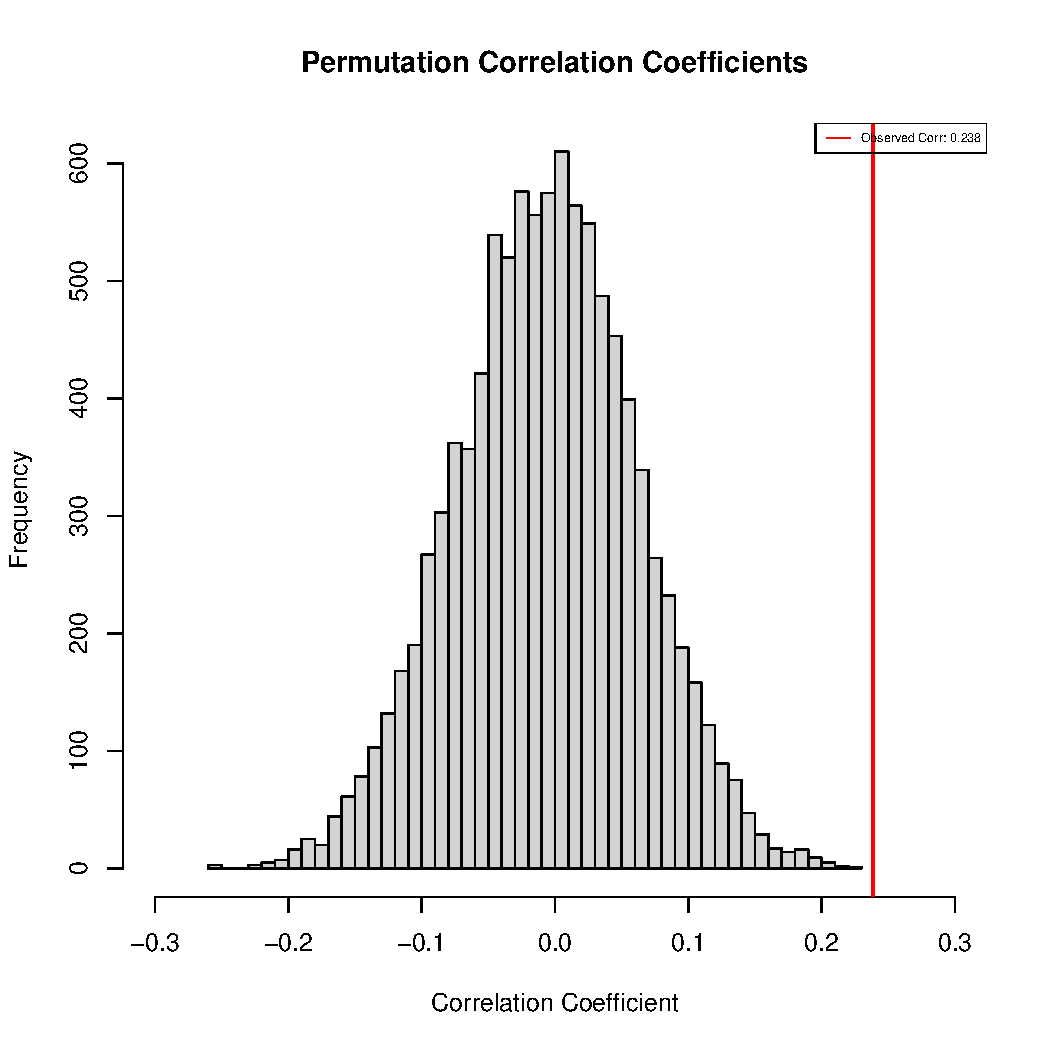
\includegraphics[width=0.8\textwidth]{../results/correlation_histogram.pdf}
\caption{Histogram of Permutation Correlation Coefficients}
\end{figure}

\section{Conclusion}
The study reveals a statistically significant, albeit mild, positive correlation in annual mean temperatures across consecutive years in Florida. This finding underscores the importance of considering recent temperature trends in long-term climate modeling and policy making.

\end{document}
